\section{Application: Perspective rendering}

As an application of linear transformations, we consider the problem
of perspective rendering. Imagine some object has been described by
coordinates in 3-dimensional space, and we wish to make an image of
the object as it would be seen by a human eye or by a camera. The
process of computing such an image is known as \textbf{rendering}%
\index{rendering}.

Conceptually, the rendering process makes use of a \textbf{camera}%
\index{camera}, which we will assume is located at the origin of a
3-dimensional coordinate system called the \textbf{camera coordinate
  system}%
\index{camera coordinates}, and an \textbf{image plane}%
\index{image plane}%
\index{plane!image plane}, which we will assume is the plane $z=1$ in
camera coordinates. The 3-dimensional space also contains one or more
objects that we wish to render. We can consider the object to be
described by a set of points. For each point $\vect{p}$ on the object,
draw a straight line from $\vect{p}$ to the camera, and let
$\vect{p}'$ be the point where this line intersects the image
plane. The point $\vect{p}$ of the object is rendered as the point
$\vect{p}'$ in the image. This process is illustrated in the following
figure:
\begin{equation*}
  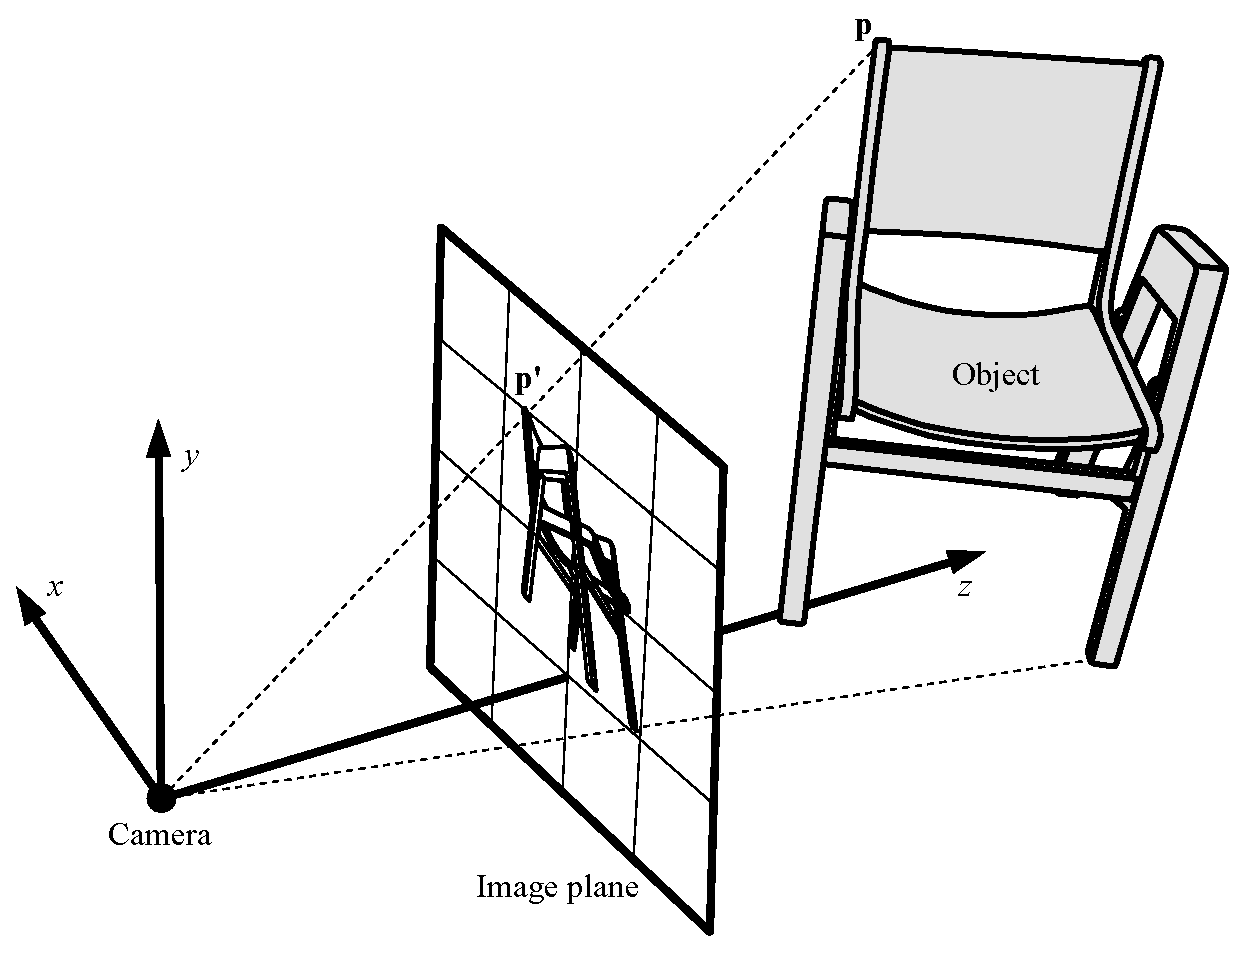
\includegraphics[width=0.90\textwidth]{figures/perspective-chair}
\end{equation*}
